%----------------------------------------------------------------------------------------
%	PACKAGES AND OTHER DOCUMENT CONFIGURATIONS
%----------------------------------------------------------------------------------------

\documentclass[paper=a4, fontsize=11pt]{scrartcl} % A4 paper and 11pt font size

\usepackage[margin=1.0in]{geometry}	%for some reason, looks beter. 

\usepackage[T1]{fontenc} % Use 8-bit encoding that has 256 glyphs
\usepackage{fourier} % Use the Adobe Utopia font for the document - comment this line to return to the LaTeX default
\usepackage[english]{babel} % English language/hyphenation
\usepackage{amsmath,amsfonts,amsthm} % Math packages

\usepackage{lipsum} % Used for inserting dummy 'Lorem ipsum' text into the template

\usepackage{sectsty} % Allows customizing section commands
\allsectionsfont{\centering \normalfont\scshape} % Make all sections centered, the default font and small caps

\usepackage{fancyhdr} % Custom headers and footers
\pagestyle{fancyplain} % Makes all pages in the document conform to the custom headers and footers
\fancyhead{} % No page header - if you want one, create it in the same way as the footers below
\fancyfoot[L]{} % Empty left footer
\fancyfoot[C]{} % Empty center footer
\fancyfoot[R]{\thepage} % Page numbering for right footer
\renewcommand{\headrulewidth}{0pt} % Remove header underlines
\renewcommand{\footrulewidth}{0pt} % Remove footer underlines
\setlength{\headheight}{13.6pt} % Customize the height of the header

\numberwithin{equation}{section} % Number equations within sections (i.e. 1.1, 1.2, 2.1, 2.2 instead of 1, 2, 3, 4)
\numberwithin{figure}{section} % Number figures within sections (i.e. 1.1, 1.2, 2.1, 2.2 instead of 1, 2, 3, 4)
\numberwithin{table}{section} % Number tables within sections (i.e. 1.1, 1.2, 2.1, 2.2 instead of 1, 2, 3, 4)

\setlength\parindent{0pt} % Removes all indentation from paragraphs - comment this line for an assignment with lots of text

%----------------------------------------------------------------------------------------
%Personal Packages and File Dependencies 
%----------------------------------------------------------------------------------------	

\usepackage{graphicx}	%insert graphics
\usepackage{microtype}	%improves spacing
\usepackage{float}		%H postion	
\usepackage{caption}	%caption w/o : 	
\usepackage{framed}		%creates frames
\usepackage{enumitem}
\usepackage{nag}

\usepackage{listings}	%insert sourcecode
\usepackage{color}
\usepackage{pdfpages}	%include PDF pages

\usepackage{bigstrut}	%exce2latex table packages
\usepackage{rotating}
\usepackage{multirow}
\usepackage{booktabs}
%\usepackage[framed]{mcode}

\usepackage{cleveref}	%cooler references, needs to be last
\usepackage[bookmarks]{hyperref}
\graphicspath{{../Figures/}{../figures/}} % This automatically connects to the figure folder

%----------------------------------------------------------------------------------------
%	TITLE SECTION
%----------------------------------------------------------------------------------------

\newcommand{\horrule}[1]{\rule{\linewidth}{#1}} % Create horizontal rule command with 1 argument of height

\title{	
\normalfont \normalsize 
\textsc{TEMPLE UNIVERSITY COLLEGE OF ENGINEERING | ECE 3623 | SPRING 2015} \\ [25pt] % Your university, school and/or department name(s)
\horrule{0.5pt} \\[0.4cm] % Thin top horizontal rule
\huge Computer Assignment (CA) No. 8: 
Central Limit Theorem \\ % The assignment title
\horrule{2pt} \\[0.5cm] % Thick bottom horizontal rule
}

\author{Tyler Berezowsky} % Your name

\date{\normalsize\today} % Today's date or a custom date 
\usepackage{listings}
\usepackage[normalem]{ulem}
\lstset{
  numbers=left,
  language=Python,
  showstringspaces=false
}
%\usepackage{mcode}

\begin{document}
\maketitle % Print the title

\section{Problem Statement} 
%Summarize the problem statement in one paragraph. Clearly state what the knowns are and what unknowns you must find.
The goal of this assignment is to demonstrate an application of the Central Limit Theorem.
The tasks to be accomplished are:
\begin{enumerate} 
\item Generate a sum of uniformly distributed mutually independent random variables:
\begin{equation}
S_n = X_1 + X_2 + \dots + X_n
\end{equation}
Write this as a function in MATLAB with arguments that include the number of random variables (n), the number of total samples generated (N), and the range of the uniform random number generator (e.g., min=-1, max=1).

\item In the main part of your program, write a loop for n=1,100, and call this function for N=10,000 with a range of [-1,1]. For each iteration, compute the mean and variance of the output sequence, Sn, and plot the RMS error between a Gaussian fit of this distribution and the actual distribution (I hope you are using your code from a previous homework assignment in a function!).

\item Plot the RMS error as a function of the value of n. Also display the actual distribution and overlay its Gaussian fit for n=1, n=10 and n=100.

\item  Consider the following technique for generating a Gaussian distribution from a uniform random number generator: \\ \verb|http://en.wikipedia.org/wiki/Box\E2\80\93Muller\_transform|.\\
Generate N=10,000 random numbers using this technique, estimate a pdf, and compare the result using the RMS error to (2) for n=10, N=10,000, range=[0,1]. Time the code in both cases using MATLABs built-in timing tools. Which technique gives the better fit? Which technique is faster? How low can you set n to get comparable performance in both time and RMS error?
\end{enumerate}
Discuss how (1)-(3) demonstrates the Central Limit Theorem.


\section{Approach and Results} 
%Describe your approach to finding the unknowns. Use numbered figures, tables and equations where necessary.

\subsection{Tasks 1 to 3} 
A function \verb|uniformsum(n, N, a, b)| was constructed which generates $n$ random variables with a length of $N$ and limits equal to $[b,a]$. This function was called with $n=[1, 100]$ and $N = 10000$,  and for each value of $n$ the PDF calculated from the resulting vector $S_n$ The normal distribution was also fitted per $n$. The RMS error, defined below, was calculated for each value of $n$ and plotted as a function of $n$ where $f_1$ is the fitted normal distribution and $f_2$ is the PDF of $S_n$. This can be seen in figure~\ref{fig: p1}. 
\begin{equation}
RMS_{error} = \sqrt{MSE} = \sqrt{E[(f_1 - f_2)^2]}
\end{equation}
 
\begin{figure}[H] 
	\centering 
	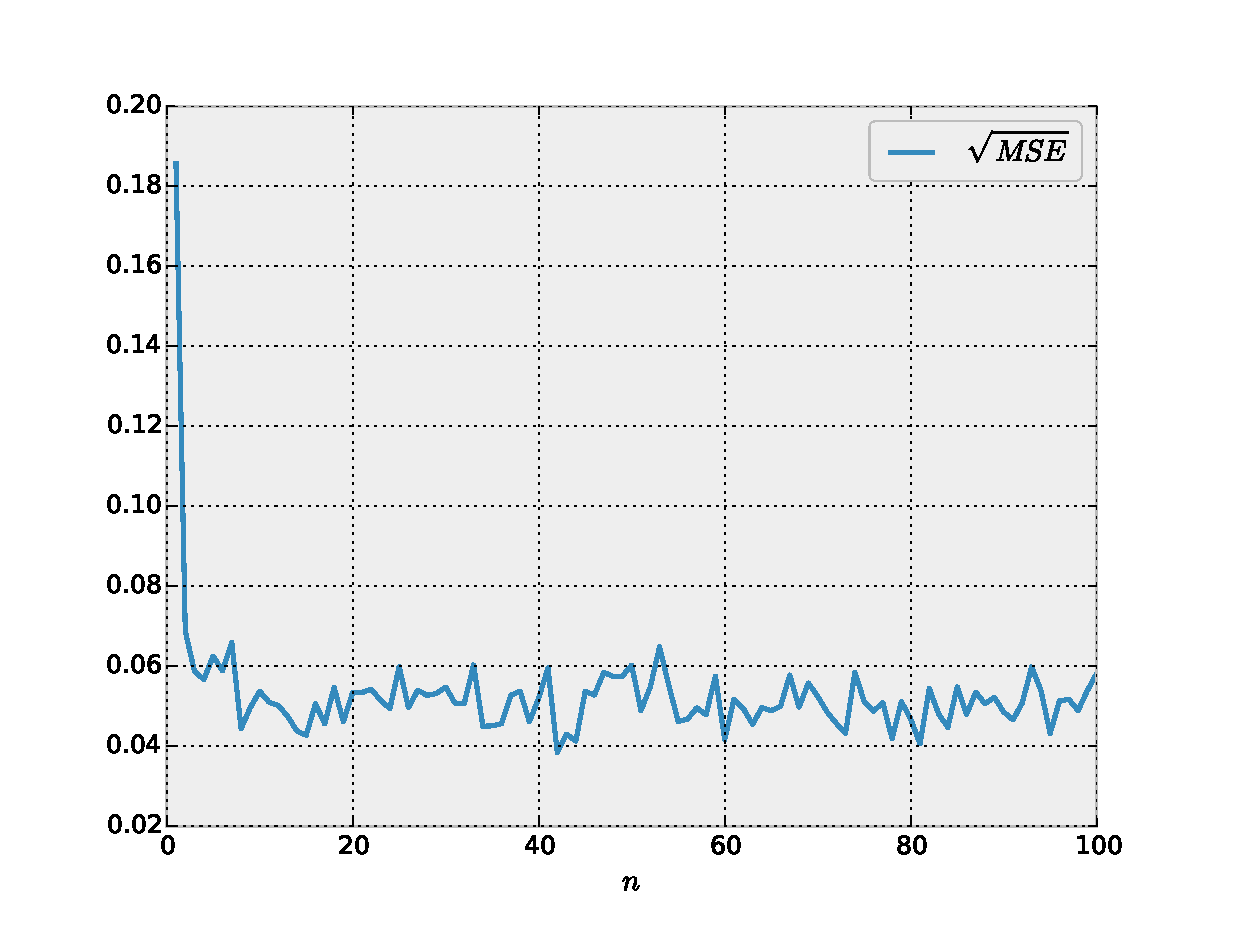
\includegraphics[width=\linewidth]{figure_1}
	\caption{$\sqrt{MSE)}$ as a function of $n$}
	\label{fig: p1} 
\end{figure}

Interestingly, the $\sqrt{MSE}$ appears to converge between 0.06 and 0.04 after only ten iterations which infers diminishing returns after $n = 10$. Plots of the $PDT_{S_n}$ are displayed in figure~\ref{fig: p2} with $n = \{1, 10, 100\}$. As previously stated,  $n$ is equal to number of  uniformly distributed random variables of length $N$ being summed to generate $S_n$. \\

When $n = 1$,  $S_n$ represents a single random variable, and is thus a uniform distribution. This is illustrated in the top subplot. When $n=10$, $S_n$ represents the sum of 10 random variables. As the middle subplot illustrates, the distribution of $S_n$ now approaches a normal distribution. When $n=100$, $S_n$ represents the sum of 100 random variables. The PDF of $S_n$ is displayed in the bottom subplot, and as predicted by error plot in figure~\ref{fig: p1}, the distribution appears identical in approximation to the fitted normal distribution of $S_n$. 

\begin{figure}[H] 
	\centering 
	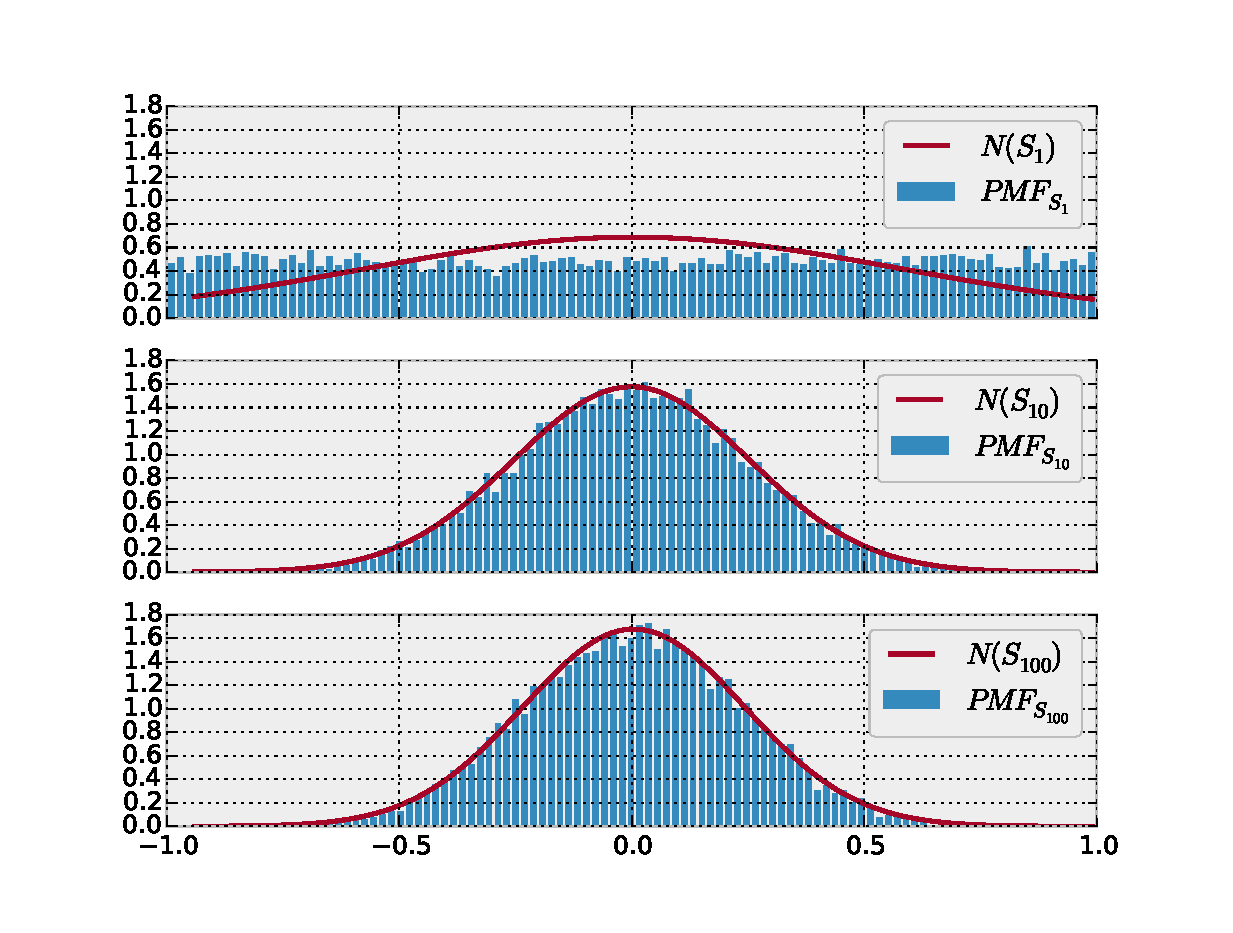
\includegraphics[width=\linewidth]{figure_2}
	\caption{Histogram of $S_n$ and fitted normal distribution}
	\label{fig: p2} 
\end{figure}

\subsection{Task 4} 
The Box-Muller method was utilized to generate a normally distributed random variable and timed against the calculation for $S_n$ with $n = [1,10]$. The Box-Muller method is described below where $Z_0$ and $Z_1$ are normally distributed random variables, and $U_1$ and $U_2$ are independent uniformly distributed random variables: 
\begin{eqnarray}
Z_0 = R\cos(\theta) = \sqrt{-2\ln{U_1}}\cos{(2\pi U_2)} \\
Z_` = R\sin(\theta) = \sqrt{-2\ln{U_1}}\sin{(2\pi U_2)}
\end{eqnarray}
The Box-Muller method and calculation for $S_n$ was trialed 10 times for each value of $n$. The result was averaged per $n$. The RMS error between the fitted normal distribution, $S_n$, and the Box-Muller method was also determined. The results are illustrated in figure~\ref{fig: p3}. \\ 

The top subplot illustrates the time for each function given $n$. As expected the time to complete the calculation for $S_n$ increases with $n$. The Box-Muller method is constant as $n$ is irrelevant for the calculation. The functions intersect when $n \approx = 2$. The bottom subplot illustrates the error between the normal distribution and the PDF of the Box-Muller method and $S_n$. As previously described, the RMS between $S_n$ and the normal decreases with $n$. The Box-Muller method is constant because $n$ is irrelevant in the calculation. The error of the Box-Muller method is consistently lower than that of $S_n$ as seen for $n = [1, 10]$. Figure~\ref{fig: p1} displays that the error converges to 0.06 and 0.04 as $n$ increases beyond 10, therefore it can be expected that the Box-Muller will be more accurate despite increasing values of $n$. Further trials would have to be attempted to confirm the previous assumption, but if error for $S_n$ does decrease with $n$, the time required would be magnitudes larger than that of the Box-Muller method. 

\begin{figure}[H] 
	\centering 
	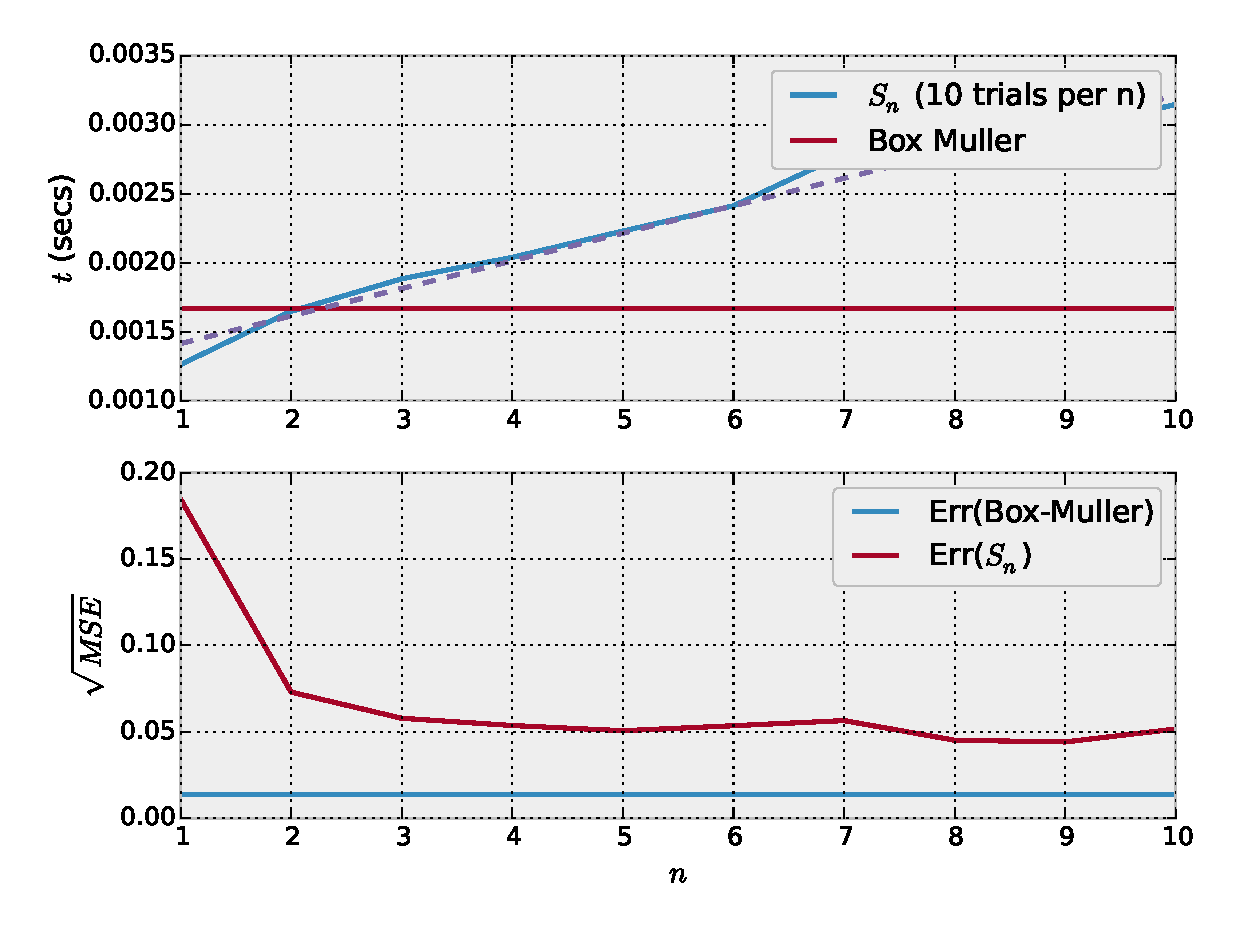
\includegraphics[width=\linewidth]{figure_3}
	\caption{Comparison of calculation for $S_n$ and Box-Muller method for the generation of a random normally distributed vector.}
	\label{fig: p3} 
\end{figure}

\section{Source Code} 
%Show and briefly explain your MATLAB code.
\lstinputlisting[frame=none]{../Python/ca_08_01.py}

\section{Conclusions} 
%Summarize what you found.
Due to the Central Limit Theorem, as $n$ is increased the sum of $n$ uniformly distributed random variables approaches a vector which is normally distributed. Central Limit Theorem: The arithmetic mean of a sufficient number of independent random variables will be \textit{approximately} normally distributed given the random variables are identically distributed.\footnote{http://en.wikipedia.org/wiki/Central\_limit\_theorem} \\ 

This theorem can be utilized to generate a random normally distributed variable, but as displayed takes considerable effort in comparison to other methods such as the Box-Muller method. Further exploration is required to understand why the RMS error appears to converge as $n$ increases. The proof of the Central Limit Theorem states given any random variable $Y$ with $E(Y) = 0$ and $var(Y) = 1$ summed $n$ times as $\lim_{n \to \infty}$ the approximation approaches $e^{-t/2}$ which would be equal to $N(0, 1)$. Therefore, error should decrease as $n$ increases. 

\end{document}